\section{تاریخچه‌ی پویانمایی سنتی}

پویانمایی سنتی که با اسم‌های مختلفی مانند "پویانمایی مرسوم" ، "پویانمایی سل‌ای"و "پویانمایی بادست" شناخته می‌شود، روشی 
غالب برای تولید فیلم‌های پویانمایی‌شده در حدود قرن 20 میلادی بود.
در این روش، به صورت کلی پویانمایی به وسیله‌ی نقاشی با دست به وجود می‌آید.
درواقع هر فریم از فیلم، یک عکس از نقاشی است و
برای به وجود آوردن توهم حرکت، هر نقاشی اندکی با نقاشی قبلی خود تفاوت دارد.

برای تولید پویانمایی سنتی، از روش‌های مختلفی استفاده می‌شد. در اینجا به بررسی
سه روش استفاده شده در پویانمایی سنتی می‌پردازیم.
 
\subsection{فریم‌های کلیدی و درمیان}
از آنجایی که تولید پویایی با دست و کشیدن نقاشی کار بسیار طولانی‌ای بود، برای اینکه وقت پویانمای‌های ارشد 
ذخیره شود، این پویانماها فریم‌های اصلی یک حرکت را بر روی کاغذ ترسیم می‌کردند و 
فریم‌های میانی را پویانماهای جوان پر می‌کردند.
  
\begin{figure}[ht]
	\centerline{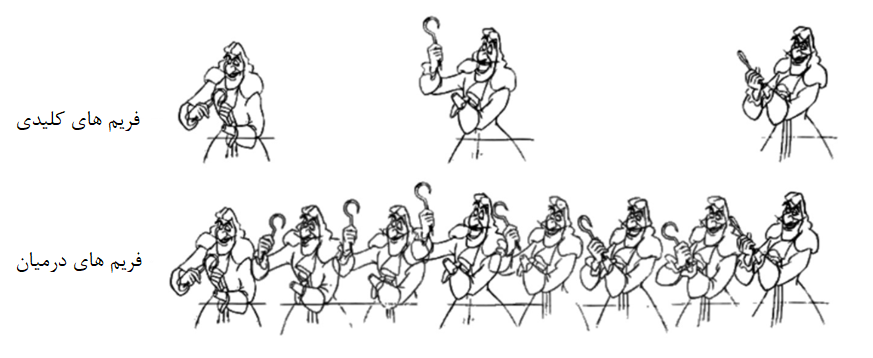
\includegraphics[width=\textwidth,height=\textheight,keepaspectratio]{Figures/Ch1/KeyframeAnimation.png}}

	\caption{فریم‌های کلیدی و درمیان \cite{Keyframeberkeley}}
	\label{fig:KeyframeAnimation}
\end{figure}

\subsection{چشم‌انداز چندمنظوره}

استفاده از چشم‌انداز چندمنظوره روش دیگری بود که در پویانمایی سنتی استفاده می‌شد.
هماطور که از تصویر زیر مشخص است، برای نمایش یک محیط از یک چشم‌انداز استفاده می‌شد.
این چشم‌انداز می‌توانست نشان دهنده‌ی قرارگیری محیط در فواصل مختلف باشد. در این صورت، زمانی که 
دوربین در صحنه حرکت می‌کرد این توهم را در مخاطب ایجاد می‌کرد که گویی در محیط در حال حرکت هستیم.

\begin{figure}[ht]
	\centerline{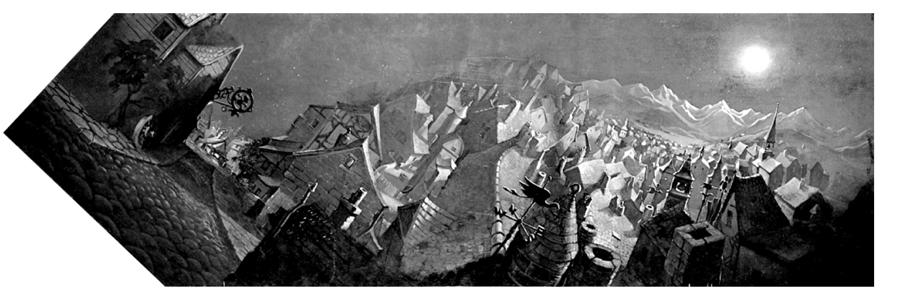
\includegraphics[width=\textwidth,height=\textheight,keepaspectratio]{Figures/Ch1/Panorama.png}}

	\caption{چشم‌انداز چندمنظوره \cite{Wood1997Multiperspective}}
	\label{fig:Panorama}
\end{figure}


\subsection{لایه‌های مختلف}

با استفاده از این روش، پویانما‌ها یک صحنه را به چند قسمت مختلف تقسیم می‌کردند.
به عنوان مثال لایه‌های مختلفی برای هر شخصیت درون صحنه استفاده می‌شد. علاوه بر این یک لایه نیز برای تصویر پس‌زمینه استفاده می‌شد.
از آنجایی که این لایه‌ها یک صفحه‌ی شفاف هستند، بنابراین می‌توان لایه‌‌ها را 
بر روی هم انباشته کرد و با تصویر برداری از بالا، تمام صحنه را تصویربرداری کرد.
این روش در تصویر 
\ref{fig:DifferentLayers}
آورده شده است.

\begin{figure}[ht]
	\centerline{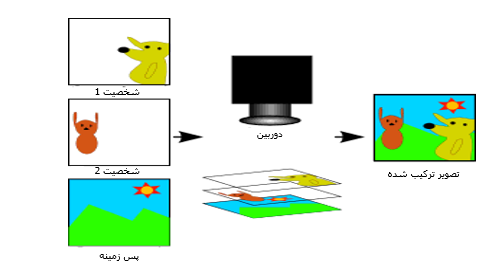
\includegraphics[width=\textwidth,height=\textheight,keepaspectratio]{Figures/Ch1/DifferentLayers.png}}

	\caption{لایه‌های مختلف\cite{AnimationCellsWikipedia}}
	\label{fig:DifferentLayers}
\end{figure}

\section{پویانمایی کامپیوتری}

اگر بخواهیم نگاهی به تاریخچه‌ی پویانمایی کامپیوتری بیاندازیم، مشاهده می‌کنیم که 
در حدود دهه‌ی 1980 میلادی شرکت دیزنی به عنوان یکی از اولین شرکت‌های جهان، شروع به 
دیجیتالی کردن خط لوله‌ی تولید پویانمایی سنتی خود کرد.
در این دیجیتال‌سازی بسیاری از روش‌ها و ایده‌‌های استفاده شده در پویانمایی سنتی،
به‌کار گرفته‌شد.
اولین مقالات این حوزه توسط آقای جان لستر از کارمندان پیکسار به عنوان 
"اصول پویانمایی سنتی به‌کار رفته در پویانمایی کامپیوتری سه‌بعدی"
ارائه شد.
در این مقاله اصول اولیه پویانمایی سنتی دوبعدی ترسیم شده با دست
و کاربرد آن‌ها در پویانمایی کامپیوتری سه‌بعدی شرح داده شده است.
\cite{Lasseter1987animation}
 
پویانمایی کامپیوتری تنها محدود به دنیای سینما و فیلم‌های پویانمایی نمی‌شوند و به دنیای
بازی‌های کامپیوتری نیز ورود پیدا کرده‌اند. بازی‌های کامپیوتری سعی می‌کنند دیوار میان تماشاگران و فیلم را بشکنند و 
با تعاملی بودن و دادن آزادی عمل به بازیکن، سعی می‌کنند داستان را به گونه‌ای تعریف کنند که گویی بازیکن یکی از شخصیت‌های اصلی داستان است.
پویانمایی در بازی‌های کامپیوتری اهمیت بسیار بالایی دارد زیرا همانطور که گفته شد باعث 
جان بخشیدن به شخصیت‌ها می‌شود که اهمیت بسیار بالایی برای جلب توجه بازیکنان در هنگام داستان‌سرایی دارد.

با پیشرفت تکنولوژی، همراه با استفاده از روش‌های گذشته، روش‌های جدیدتری برای تولید پویانمایی توسعه یافته‌است که 
در ادامه به چند مورد از آن‌‌ها می‌پردازیم.

\subsection{فریم‌های کلیدی و درمیان}

همانطور که اشاره شد در پویانمایی کامپیوتری از روش‌های موجود در 
پویانمایی سنتی استفاده شده است. در اینجا نیز فریم‌های کلیدی 
یک حرکت، توسط پویانماها به وجود می‌‌آیند ولی فریم‌های میانی به جای اینکه توسط پویانماها به وجود آیند،
توسط کامپیوتر با استفاده از روش های درون‌یابی به وجود می‌آیند.

\subsection{رویه}

در این روش، حرکت بر اساس یک الگوریتم بیان می‌شود.
درواقع کلیپ‌های پویانمایی در این نوع پویانمایی، توابعی با تعداد کمی از متغیر‌ها هستند.
به عنوان مثال یک تابعی را درنظر بگیرید که با گرفتن ورودی ثانیه، دقیقه و ساعت، 
یک شئ ساعت را خروجی دهد که عقربه‌هایش در جای مناسب با توجه به ورودی‌ها قرار گرفته باشد.
حال می‌توان با تغییر ورودی‌ها حرکت ساعت را شبیه‌سازی کنیم.

\subsection{مبتنی بر فیزیک}

پویانمایی مبتنی بر فیزیک پلی میان دنیای پویانمایی با 
دنیای واقعی است. در این روش با نسبت دادن ویژگی‌های فیزیک به اشیاء سه‌بعدی و سپس حل‌کردن
فرمول‌های فیزیک مانند فرمول حرکت یا فرمول‌های نیوتن،
فیزیک شبیه سازی می‌شود.
پویانمایی‌های مبتنی بر فیزیک شخصیت را قادر می‌سازد تا حرکت‌های خود را 
به صورت پویا با محیط تنظیم کند.

\subsection{ضبط حرکت
\protect \LTRfootnote{Motion Capture}}

به فرآیند ثبت و دیجیتالی‌کردن حرکت یک شئ یا شخص، ضبط حرکت گویند.
ضبط حرکت توسط دوربین‌های مادون قرمز که تعدادی زیادی از آن‌ها در صحنه‌ی ضبط قرار دارند، صورت می‌گیرد.
این دوربین‌ها به صورت شبکه به یکدیگر متصل هستند و پس از کالیبره شدن، آماده‌ی استفاده هستند.
این دوربین‌ها با استفاده از نشانگر‌های سفیدی که بر روی لباس بازیگران 
ضبط حرکت قرار دارد، داده‌های مورد نیازشان را دریافت می‌کنند.
قابل ذکر است این نشانگر‌ها بازتابنده‌ی مادون قرمز هستند که توسط دوربین‌ها دریافت می‌شود.
در نهایت پویانماها به پاکسازی و پردازش این داده‌ها پرداخته تا آن را 
برای استفاده‌ی شخصیت‌های سه بعدی آماده کنند.


